\chapter{Monitorização de processos}
\label{cap:trabrelacionado}
 
\section{Visão geral} \label{sect:descricao}

Pode ser necessário recorrer à monitorização para se compreender o comportamento das aplicações.
Esta permite-nos obter dados relevantes sobre os recursos utilizados, de modo a proporcionar-nos um conhecimento mais profundo do seu comportamento.
As informações recolhidas podem servir para analisarmos comparativamente o desempenho de diferentes versões de uma mesma aplicação, porquanto ao conseguir-se obter dados da utilização do \textit{cpu}, da memória, dos dispositivos de \textit{IO}, etc, é possível compreender o comportamento dinâmico das aplicações.
Daí ser comum a utilização da monitorização como auxiliar na depuração de programas.~\cite{DuartePhd05}.

\subsection{Obtenção de informação}\label{sect:instrumentation_overview}

Os dados relativos ao comportamento das aplicações, obtidos de diferentes fontes, são coligidos e posteriormente analisados por ferramentas especializadas.
Existem diferentes formas de coligir, visualizar e até interactuar com as ferramentas de monitorização, cada uma com as suas especificidades e capacidades próprias.

Tendo em vista o conhecimento e um melhor aproveitamento das capacidades de cada uma, são apresentadas as diferentes formas de análise / avaliação:

Se considerarmos como referência a visualização da história dos eventos, podemos analisá-los de duas formas distintas:
 
\subparagraph*{Online -}
Enquanto decorre a monitorização da aplicação é possível observar os dados que são recolhidos pelo monitor.
Como os eventos estão a ser recolhidos e visualizados em simultâneo, apenas podemos observar a história até ao momento, mas temos uma baixa latência entre os acontecimentos e a sua observação.

\subparagraph*{Offline ou \textit{Post-Mortem} - }

A história do programa é analisada após este se ter completado daí a designação \textit{Post-Mortem}.
Este método permite-nos analisar integralmente a sua história e coleccioná-la.
Permite análises mais completas e computacionalmente mais exigentes.

Se a monitorização necessitar de interactividade do utilizador, é possível defini-la de duas formas:

 \subparagraph*{Activa - }

Por iniciativa explícita do utilizador, é possível inquirir o sistema de monitorização sobre o estado da computação ou mesmo alterá-la.
Este método, por vezes descrito como \textit{computacional steering}, é a forma com maior interactividade, uma vez que permite ir analisando e modificando os parâmetros da monitorização ou mesma da aplicação.

\subparagraph*{Passiva - }
Esta forma de monitorização é especialmente utilizada em ambientes onde é relevante a obtenção da totalidade dos dados e apenas no final nos debruçarmos sobre a sua análise.
Esta forma é designada de passiva, por o utilizador não ter intervenção na forma como os dados estão a ser obtidos, o que reduz a perturbação do sistema. 

A instrumentação pode ser de dois tipos: a estática e a dinâmica, cada uma com as suas características próprias.

\subparagraph*{Estática - }

Na instrumentação estática o código instrumentado é definido em tempo de compilação, ou utilizando bibliotecas próprias para o efeito, como a utilização da função \textit{assert}, que define os pontos a serem monitorizados.
Durante a execução não podem ser adicionados ou removidos pontos de análise.

\subparagraph*{Dinâmica - }

Em contraste com a instrumentação estática está a dinâmica.
É mais complexa e permite a inserção e remoção dos pontos a serem monitorizados.
O dinamismo verifica-se pela ausência do ciclo $introduzir ponto\rightarrow compilar programa\rightarrow executar\rightarrow remover ponto$.
A utilização de pontos de instrumentação dinâmica, pode ajudar a reduzir o grau de perturbação, uma vez que apenas são definidos os que se desejam observar.
Tal pode ser efectuado no início da execução ou durante a sua execução, criando, alterando, destruindo os pontos de observação sobre os recursos monitorizados.


\subparagraph*{
%Recolha de dados
}
A recolha de informação, é uma das componentes mais sensíveis relativamente ao grau de perturbação da monitorização.
Em geral os pontos de instrumentação levam a que os dados sejam armazenados num \textit{buffer} em memória.
Caso exista algum evento que indique que o \textit{buffer} se encontra cheio ou por acção explícita do utilizador tal é transferido para a interface com o utilizador que a visualiza ou armazena em memória persistente, para posterior análise.

\subparagraph*{
%Grau de perturbação
}
Existe claro a preocupação de que o sistema a ser monitorizado tenha um baixo grau de perturbação, pois pode levar à alteração dos resultados obtidos e mesmo a comportamentos diferentes da aplicação (especialmente perante execuções concorrentes).
Daí que, diversas abordagens foram criadas, para reduzirem o impacto da monitorização num sistema em produção.
Uma destas abordagens traduz-se na utilização de instruções especializadas, de que alguns processadores dispõem para \textit{debug}, de modo a utilizar os recursos que mais se adequem à monitorização.
Estes métodos, nem sempre são utilizados, devido à sua dependência da arquitectura, o que dificulta a sua portabilidade.
Com vista a minimizar a perturbação, alguns sistemas de monitorização utilizam uma técnica de amostragem, que permite obter indicações sobre os estado da computação a cada intervalo de tempo.
Esta técnica, em oposição à criação de um traço de execução, permite obter dados sobre os recursos apenas por amostra, limitando à partida a perturbação, enquanto que na criação de um traço de execução, é possível obter a totalidade dos eventos de forma a criar uma história completa, mas pode levar a uma grande sobrecarga do sistema perante uma grande taxa de eventos.

\paragraph*{
%Apresentação dos dados recolhidos
}
No entanto, capturar estes dados oriundos da monitorização pode revelar-se insuficiente, se não dispusermos de uma ferramenta onde estes possam ser tratados, de modo a obtermos análises mais completas e relacionar com os detalhes de funcionamento da aplicação.
Este não será o foco deste trabalho.

\subsection{Monitorização de Rede}\label{sub:network_monitoring}

Em geral, as ferramentas de monitorização da interacção do processo com o exterior, são baseadas na captura de pacotes de forma passiva.
As ferramentas capturam os pacotes que fluem na rede, para posterior análise ao tráfego, que pode incidir sobre a largura de banda utilizada, principais protocolos, eventuais problemas de segurança, etc.

\subparagraph*{Dinamismo das aplicações - }
Como o anteriormente referido, as aplicações são dinâmicas e a este dinamismo se devem algumas dificuldades com que nos deparamos, ao monitorizar as aplicações.

Relativamente à monitorização das interacções com o exterior, utilizando os mecanismos do sistema de operação, este dinamismo é um factor chave, pois existem dificuldades na forma de identificar os fluxos pertencentes a um processo face aos restantes irrelevantes na nossa análise.

\subparagraph*{Formas de reduzir o volume de dados utilizando filtros - }
A utilização de filtros na captura do tráfego que circula na rede, é uma forma eficiente de apenas se obterem os dados relevantes, com vista à satisfação dos nossos objectivos e são particularmente importantes, quando o volume de dados que circula na rede é extremamente elevado.
Tendo em vista a eficiência, estes filtros são implementados no núcleo do sistema de operação, baseando-se em regras simples, que podem ser combinadas para contemplar situações mais complexas.

\subparagraph*{Dificuldade de criação e alteração de filtros - }
Os filtros actualmente suportados para capturar pacotes no \textit{Linux}, são definidos \textit{a priori}, não existindo forma eficiente de os alterar dinamicamente, uma vez que a captura tem de ser interrompida a fim de ser criado um novo filtro, posteriormente aplicado, procedendo-se em seguida à retoma da captura dos pacotes, de acordo com as novas regras.

\subparagraph*{Filtros mais complexos e inteligentes - }
De forma a aumentar o desempenho da captura de pacotes, os filtros são aplicados o mais cedo possível, ou seja, logo que chegam à interface de rede.
Face a esta situação, o tipo de filtros que se podem aplicar têm de ser simples, baseados apenas no conteúdo do pacote.
Quando os filtros são demasiado complexos, os módulos do núcleo têm de passar grande parte da informação para as camadas superiores, de forma a puderem ser aplicados filtros mais elaborados, que analisam um nível mais abstracto da informação, presente no \textit{payload} dos pacotes, ou a relacionam com outra informação, para obterem apenas os dados relevantes.

\subparagraph*{Técnicas para o aumento de desempenho}
% \todo{performance ou desempenho}
Diferentes técnicas têm vindo a ser desenvolvidas para aumentar a performance de monitorização das interfaces de rede.
Como já referido, o aumento da sobrecarga é muito penalizante, daí que esta deva ser mantida bastante reduzida, o que contribuirá para aumentar o desempenho da captura.

Um exemplo é nova \textit{API} de atendimento de interrupções criada com este propósito, e encontra-se analisada na subsecção \ref{par:NAPI}.

Hoje em dia a utilização de máquinas equipadas com processadores \textit{multi-core} é uma realidade, daí que a sua utilização permita ultrapassar algumas dificuldades sentidas na captura de pacotes.
Se for os processadores \textit{multi-core} atenderem em parelelo as diversas interrupções, originadas pelo envio ou recepção de pacotes, o desempenho da rede é passível de ser aumentado.
No entanto, revela-se díficil atingir este paralelismo para todas as interfaces de rede, pois nem todas estão preparadas para beneficiar de arquitecturas com múltiplos \textit{cores}.

\section{Sistemas de monitorização no núcleo do \textit{Linux}}\label{sect:instrumentacao_casos_linux}

Como o anteriormente analisado na secção \ref{sect:instrumentation_overview} referente à monitorização, esta secção é dedicada à apresentação das diferentes ferramentas de monitorização do núcleo de sistema do \textit{Linux} sendo as mais recentemente utilizadas neste sistema de operação.
Neste documento constam apenas mecanismos e ferramentas de monitorização dinâmicas, pois apenas estas são desejadas para utilização na criação de uma componente de monitorização de rede orientada ao processo.
De entre as ferramentas de monitorização dinâmica analisadas é possível agrupa-las em duas categorias: eventos pré-definidos e instrumentação dinâmica.
Na categoria suporte à monitorização existem dois sistemas mais relevantes: o \textit{KProbes} e o \textit{Linux Kernel Stace Tracer}, enquanto que para a lista de eventos foram verificados o \textit{Linux Trace Toolkit} e o \textit{OProfile}.
Estes sistemas 4 sistemas são apresentados em seguida nas suas categorias.

\subsection{Eventos pré-definidos}

Nesta categoria encaixam-se duas ferramentas o \textit{Linux Trace ToolKit} e o \textit{OProfile}.
Em cada uma destas ferramentas a monitorização é efectuada sobre pontos previamente definidos, não permitindo a adição de novos pontos de monitorização.
Cada um destas ferramentas analisa todo o sistema, sendo a filtragem extra dos eventos efectuada em nível utilizador.
Por isso a lista de eventos pode parecer uma limitação, mas uma vez que estas ferramentas analisam todo o sistema, deixa de o parecer.

\subsubsection{Linux Trace ToolKit}\label{cap:linux_trace_toolkit_overview}

% O Linux Trace Toolkit é uma ferramenta de ``tracing''
% Utiliza o Klog com repositorio da informação obtida do kernel.
O \textit{Linux Trace ToolKit} é uma ferramenta um pouco mais antiga que o \textit{KProbes}, constituída por quatro componentes: o \textit{Kernel Patch}, o \textit{Kernel Module} o \textit{Trace Daemon} e o \textit{Data Decoder}, foi substituída pelo \textit{Linux Trace Toolkit New Generation} que se apresenta em seguida.

% Nesta versão a comunicação entre o kernel e aplicação em user space é efectuada utilizando o relayfs.
% O RelayFs é um sistema de ficheiros para comunicação entre o código dentro e fora do núcleo de operação.

O \textit{Linux Trace Toolkit New Generation}, e permite utilizar mecanismos como o \textit{KProbes}, o \textit{Tracepoints}\cite{Mathieu2009} e \textit{Linux Kernel Markers}\cite{Mathieu2009} para efectuar as suas monitorizações.
Os \textit{Tracepoints} e Linux \textit{Kernel Markers} fazem parte da instrumentação estática pertencente ao núcleo de sistema do \textit{Linux}.

A transferência dos dados do núcleo de sistema para a aplicação, é efectuada utilizando o sistema de ficheiros virtual \textit{RelayFs}.

%A utilização desta ferramenta em sistemas de tempo real é um bom indicador da sua performance.

%\subparagraph{Linux Trace Toolkit Viewer - }\label{cap:lttv_overview}
O \textit{Linux Trace Toolkit Viewer (LTTV)} é um projecto desenvolvido em paralelo com o \textit{LTT} e \textit{LTTng}, de forma a possibilitar uma análise visual dos dados recolhidos por estas aplicações.
Esta ferramenta possibilita igualmente realizar um traço de execução, uma vez que os dados recolhidos contêm uma estampilha temporal, do momento em que foram obtidos.
 
\subsubsection{OProfile}\label{cap:Oprofile_overview}
As ferramentas anteriormente referidas utilizam mecanismos para obter um traço de execução, este difere neste facto.
Em vez de a cada evento utilizar uma função para obter os dados, apenas a utiliza decorridos um certo número de eventos.
O recurso a este critério permite ao \textit{OProfile} ser menos perturbador, uma vez que nem sempre é necessário o universo dos eventos que as ferramentas de monitorização capturam, mas tão somente uma amostra.
Deste modo ao utilizar a amostragem, o \textit{OProfile}, beneficia de um menor grau de perturbação no sistema\cite{Will:TuninProgrOProf}.
% ser menos perturbador do sistema.
% it uses data sampling ... the others don't

% outra abordagem 

\subsection{Suporte à monitorização}

Como suporte à monitorização destacam-se duas ferramentas: o \textit{KProbes} e o \textit{Linux Kernel Stace Tracer}.
Em ambos é possível definir novos pontos, funções ou eventos a serem monitorizados, não ficando restrito a funcionalidades já existentes nestas ferramentas.

\subsubsection{KProbes}\label{sect:KProbes_overview}

O \textit{KProbes} é um mecanismo de instrumentação dinâmica do núcleo do \textit{Linux}.
A \textit{API} permite que aplicações, como o \textit{DProbes} ou o \textit{SystemTap} possam aceder às suas funcionalidades.
Esta encontra-se na versão principal do núcleo do sistema \textit{Linux} desde a versão 2.6.9, o que indica tratar-se de uma ferramenta bastante estável\cite{kernel_debug_printk_on_fly,KProbesSite}.

Existem três tipos de instrumentação que podem ser efectuados: \textit{KProbe}, \textit{JProbe} e \textit{KRetProbe}.
Cada um destes três tipos é especifico de uma determinada funcionalidade.

\begin{itemize}
 \item \textbf{KProbe - }

Utilizando um \textit{KProbe} pode-se analisar a chamada de uma função ou de uma instrução.
Para analisar apenas uma instrução, tem de ser indicado o \textit{offset} relativamente à distância ao inicio da função instrumentada.
A indicação da função a instrumentar, pode ser definida recorrendo ao seu nome ou ao endereço de memória.
Múltiplos \textit{KProbe} podem ser definidos para uma mesma função ou instrução.

\item \textbf{JProbe - }

Um \textit{JProbe} destina-se a analisar os parâmetros, da função a instrumentar.
Quando é declarado um \textit{JProbe} a função de \textit{handler} tem de conter os mesmos tipos de argumentos que a função que se destina a ser instrumentada, de forma a serem monitorizadas.
 
 \item \textbf{KRetProbe - }

Este tipo de análise tem como objectivo obter o valor de retorno da função que se pretende analisar.
Para efectuar esta operação é utilizada a técnica do trampolim~\cite{Hollingsworth94dynamicprogram}, uma vez que uma função pode terminar em pontos diversos.

\end{itemize}

Para se obterem informações sobre as funções ou instruções que estão a ser monitorizadas, o \textit{KProbes} disponibiliza-as através de um ficheiro no \textit{DebugFs}.
Para utilizar o \textit{KProbes} é necessário criar um módulo para o núcleo do sistema de operação, com informações relativas às rotinas a instrumentar.
Para além destas, o módulo tem de conter igualmente os \textit{handlers} de análise, assim como outros parâmetros necessários à realização da instrumentação.
Uma vez que os módulos são escritos em linguagem C ou \textit{assembly}, foram desenvolvidas as ferramentas, \textit{DProbes} e \textit{SystemTap}.
Estas novas ferramentas de mais alto nível, ajudam no desenvolvimento de \textit{scripts}, simplificando e melhorando a segurança na utilização desta ferramenta de instrumentação (\textit{KProbes}).

Quando o módulo é inserido no núcleo de sistema, o registo dos \textit{handlers} das funções a serem instrumentadas é efectuado de forma atómica.
A execução do \textit{KProbes} não utiliza nenhum \textit{mutex} ou outra forma de controlo de concorrência, apenas funciona com a preempção desligada.
Dependendo do contexto, os \textit{handlers} podem ser executados com as interrupções desligadas.

A instrumentação, processa-se substituindo por interrupções as instruções ou funções a serem analisadas, utilizando neste caso o \textit{int 3}.
Quando possível o \textit{KProbes} utiliza instruções do processador especializadas no \textit{debug} de forma a minimizar o grau de perturbação.

Apesar de ser possível instrumentar praticamente todo o núcleo do sistema de operação, existem algumas situações que podem requerer alguma perícia na forma como são tratadas.
Quando o compilador realiza substituição de funções por código \textit{inline}, as instruções que anteriormente estavam dentro da função passam a integrar o ponto onde foram substituídas, deixando de existir um ponto de entrada na função.
Assim sendo, a função deixa de existir, impossibilitando a instrumentação destas funções.

%\subsubsection{DProbes}\label{cap:Dprobe_overview}

O \textit{DProbes} utiliza o \textit{KProbes} como suporte para efectuar a instrumentação dinâmica do núcleo de sistema.
Como a criação de pontos de análise é escrito em linguagem C ou \textit{assembly}, foi desenvolvida uma linguagem de mais alto nível de forma a simplificar  a utilização desta aplicação.

Após os dados terem sido obtidos, estes podem ser transferidos para um ficheiro, para o \textit{daemon logging} do núcleo de sistema, ou para uma porta série.
Existe igualmente a opção de interoperabilidade com o \textit{Linux Trace Toolkit}\cite{:DProbes}.

%\subsubsection{SystemTap}\label{cap:Systemtap_overview}

O \textit{SystemTap} é uma ferramenta que possibilita o desenvolvimento de módulos para o \textit{KProbes}, utilizando uma linguagem específica, de forma a ser segura e fácil de trabalhar.

Uma vez que os dados gerados estão no espaço de endereçamento de memória do núcleo, e o programa que os analisará se situa no espaço de endereçamento do utilizador, é necessário efectuar uma transferência de dados de um para outro espaço.
O \textit{SystemTap} efectua esta transferência, recorrendo à utilização do sistema de ficheiros \textit{ReplayFs}, onde é possível escrever de forma rápida, sem comprometer a segurança do sistema\cite{Donovan2007,Jones2009}.

Apesar de no pacote de aplicações desta ferramenta, existir um visualizador gráfico de dados, recolhidos pelo \textit{SystemTap}, esta só consegue analisar os \textit{TapSets} pré-definidos no \textit{SystemTap}.
Para ultrapassar esta limitação, novas ferramentas estão a ser desenvolvidas.
Uma destas ferramentas designada por \textit{bootlimn}, está actualmente a ser desenvolvida no \textit{Google Summer of Code}, com o objectivo de utilizar o \textit{SystemTap} para recolher informações sobre o arranque do sistema, agregando estes dados no formato \textit{XML}.
Os dados recolhidos, permitem visualizações gráficas do processo de inicialização do sistema, bem como da utilização de disco e \textit{CPU}.

Outro projecto conhecido como \textbf{Systemtap GUI}, que engloba o \textbf{System Tap Editor Plug-in} para a ferramenta Eclipse, é um ambiente onde podem ser analisados e visualizados os dados recolhidos pelo \textit{SystemTap}.

O \textit{SystemTap} actualmente está a ser desenvolvido por empresas de reconhecido mérito internacional, nomeadamente a \textit{Red Hat}, a \textit{IBM}, a \textit{Hitachi} e a \textit{Oracle}.

\subsubsection{Linux Kernel State Tracer}
% Linux Kernel State Tracer(LKST) records information as trace data about events in the Linux Kernel. It records various events like process context switch, send signal, exception, memory allocation, send packet, and so on. 

O \textit{Linux Kernel State Tracer(LKST)} obtém informações referentes ao núcleo de sistema, de forma a criar um traço de execução, e consegue capturar diferentes eventos como trocas de contexto, envio de sinais, alocação de memória, transmissão de pacotes, etc.

% a\subparagraph{DJProbe}
\label{cap:djprobe}
  % Este sistema é mais leve devido à forma como é feito o ``trap'' pois não usa o int 3
% Duvidas na forma como é controlado o sistema na presença de processadores maquinas com multiplos processadores.
% Não utiliza o int 3 para fazer o trap por isso segundo o artigo fica mais leve que o KProbe e o JProbe.
% DJProbe  quer dizer Direct Jump Probe faz um jmp e não usa o int 3.
Actualmente, está a ser desenvolvido um subprojecto do \textit{Linux Kernel Stace Tracer} designado por \textit{Direct Jump Probe}.
O \textit{Direct Jump Probe} é uma optimização à utilização do \textit{trap int3}, presente em alguns processadores, e que pode trabalhar em conjunto com o \textit{KProbes} \ref{sect:KProbes_overview}.
Esta optimização pode ser verificada no relatório\cite{Hiramatsu2005}.


\subsection{Comparação entre os diferentes sistemas de instrumentação}
% \todo{completar esta tabela}
\begin{table}[h!]
\begin{center}
\caption{Tabela Comparativa dos sistemas de instrumentação}
\label{tab:inst_compare}
\begin{tabular}{|l||c|c|c|}
\hline
Instrumentação & Amostragem / Traço & Análise de Parâmetros & Deamon \\
\hline
KProbes & Traço & Permite & Não necessita \\
\hline
LKST & Traço & Permite & Necessita \\
\hline
LTT & Traço & Não permite & Necessita \\
\hline
OProfile & Amostragem & Não permite & Necessita \\
\hline

\end{tabular}
\end{center}
\end{table}

Da observação da tabela \ref{tab:inst_compare} pode inferir-se que: ToDo

A tabela \ref{tab:inst_compare} permite fazer uma comparação entre algumas caracteristicas destes sistemas de instrumentação presentes no núcleo de sistema do \textit{Linux} segundo os seguintes critérios: metodologia da captura (por traço ou por amostragem), análise dos parâmetros das funções instrumentadas e a necessidade de ter um \textit{deamon} para a recolha de dados provenientes do sistema de monitorização.
Se a necessidade de ter um \textit{deamon} a executar de forma a coligir e organizar os dados, pode penalizar o desempenho do sistema, a possibilidade de analisar os parâmetros das funções instrumentadas é um ponto a favor deste.
\section{Transferência de dados}
\label{sect:kernel_user_comm}

Quando se recorre a alguma fonte para a obtenção de dados, não é imprescindível que estes sejam requeridos no sítio onde são capturados.
Assim, foram criados dois modos de transferência de dados: os internas e os externos.
No intuíto de melhorar a partilha dos recursos externos, o controlo dá-se ao nível do núcleo do sistema, pelo que parte das comunicações dos utilizadores com dispositivos externos, é efectuada através do núcleo de sistema.

%Incluir por aqui a informação de mmaps, ring buffers e afins ....
% colocar a parte interna e verificar o mmap que tb faz parte do utilizador
% verificar o mmap da parte de utilizador
%texto explicativo de interno e externo 
\subsection{Interno ao sistema}

Devido há necessidade de transferir informações entre diferentes \textit{buffers} dentro do núcleo de sistema, foram desenvolvidas novas técnicas tendo sempre como referência a minimização da sobrecarga.

De entre as diferentes técnicas de transferência interna de informação ao núcleo do sistema, merecem especial relevo:

\paragraph*{\textit{MMAP} - }

Esta técnica é implementada utilizando páginas de memória partilhadas, reduzindo as transferências e gastos de memória, proporciona a possibilidade de mapear um canal para memória potenciando assim, a partilha de dados entre diferentes processos que necessitem aceder aos dados do mesmo canal.
A possibilidade de partilha de dados de \textit{IO} é uma vertente que tem sido objecto de desenvolvimento, de forma a aumentar o desempenho, porquanto permite a partilha de dados entre um ou mais programas, e o núcleo de operação.

\paragraph*{Zero Copy - }

Esta técnica de transferência de dados sem que existam cópias dos \textit{buffers} pertencentes ao núcleo de sistema e ao espaço de utilizador, permite que os dados sejam partilhados por diferentes entidades, sem a necessidade de criação de novos \textit{buffers} e cópias de dados, uma vez que apenas são passadas as referências.

\paragraph*{Ring Buffers - }

Esta técnica consiste num aproveitamento dos recursos já alocados, mas que se tornaram desnecessários, estando desta forma disponíveis para nova utilização.
Os \textit{Ring Buffers} são utilizados tendo presente a relação custo / benefício, isto é, quando o peso da criação de novos elementos é compartivamente superior aos recursos já alocados.
É igualmente utilizada em situações de \textit{"produtor-consumidor"}, ou seja, quando é necessário manter a ordem dos elementos.

\paragraph*{NAPI - New API - }

Foi criada uma nova \textit{API} (\textit{Application Program Interface}) de atendimento de interrupções do processador, oriundos das interfaces de rede, com o objectivo de aumentar o desempenho da utilização de rede de elevado débito.
Esta nova \textit{API}, permite desligar a atenção do processador a novas interrupções, oriundas da interface de rede, durante um certo período de tempo.

Este tempo foi definido, de forma a que não se verifiquem situações de elevada latência na chegada dos pacotes às aplicações.
A forma anterior de recepção de pacotes, era efectuada de modo a atender uma interrupção por cada pacote que chegava à interface de rede, gerando assim demasiada sobrecarga no sistema.
Actualmente a arquitectura de rede, está balanceada de forma a mudar o modo de atendimento de interrupções para NAPI, caso existam demasiadas interrupções por unidade de tempo.~\cite{administrator:napi}.

Utilizando esta nova \textit{API}, é possível explorar um escalonamento mais eficiente das interrupções, em situações de intensa actividade do processador.
O \textit{NAPI} apenas pode ser aplicado nos caso em que os controladores das interfaces de rede estejam preparados para utilizar alguma forma de mitigação da interrupção, caso contrário esta \textit{API} não é aplicada.

\subsection{Com o exterior do sistema}
% {\color{red}
% \paragraph*{}
% INDICAR QUAIS OS SISTEMAS QUE OS UTILIZAM
% 
% DISTINÇÂO ENTRE OS DIFERENTES SISTEMAS
% }

Devido à necessidade de análise de estruturas e dados do núcleo de sistema, foram criados diferentes subsistemas com vista à sua satisfação.
Um destes subsistemas é o \textit{ProcFs}, que existe no núcleo de sistema do \textit{Linux} desde as primeiras versões.
Outros como o \textit{DebugFs} ou o \textit{RelayFs} são mais recentes e com novas abordagens.
%diferentes abordagens e o pq de ter de existirem estas formas

\paragraph*{}
De forma a obter informações relativas a estruturas dentro do núcleo de sistema, foram referênciados os seguintes sistemas de comunicação entre o utilizador e o núcleo, a saber:

\paragraph*{ProcFs - }\label{cap:ProcFs_overview}

Desenvolvido para obter informações relativas aos processos tem sido utilizado desde as primeiras versões do núcleo de sistema do \textit{Linux}.
Apesar de novos subsistemas como o \textit{SysFs} terem sido criados, é ainda utilizado por algumas aplicações.

\paragraph*{SysFs - }\label{cap:SysFs_overview}

Este sistema de ficheiros virtual foi desenvolvido para colmatar algumas deficiências encontradas no \textit{ProcFs}.
Estes problemas situam-se basicamente na forma como a quantidade de informação disponibilizada está distribuída sobre o \textit{ProcFs}.
Este novo sistema de ficheiros virtual, evidencia algumas restrições, designadamente na forma como são disponibilizados os dados do núcleo de sistema.
Esta limitação conduziu a que outros sistemas de ficheiros virtuais, nomeadamente o \textit{DebugFs} e o \textit{RelayFs}, fizessem a sua aparição.

\paragraph*{DebugFs - }\label{cap:DebugFs_overview}

Este sistema foi essencialmente criado a pensar nas necessidades sentidas pelos programadores.
Apesar de já existirem dois sistemas de ficheiros virtuais, o \textit{ProcFs} e o \textit{SysFs}, este tentou colmatar os problemas que se apresentavam, não obstante não se mostrar tão estruturado como o \textit{SysFs}, e com melhor organização de dados que o \textit{ProcFs}.

O sistema de instrumentação do núcleo de sistema \textit{Linux}, \textit{KProbes}, utiliza este sistema de ficheiros virtual, de forma a apresentar os pontos, onde existe instrumentação no núcleo de sistema.

\paragraph*{RelayFs - }\label{cap:RelayFs_overview}

Este sistema de ficheiros virtual foi desenvolvido tendo em mente a transferência de grandes quantidades de dados entre o núcleo de sistema e o espaço de utilizador.
O \textit{RelayFs} responde a esta exigência, fazendo uso de novas primitivas onde são mais reduzidas as zonas de controlo de concorrência\cite{Donovan2007}.

\paragraph*{NetLink - }\label{cap:NetLink_overview}
O \textit{NetLink} utiliza uma método de comunicação baseado em \textit{sockets}, para estabelecer a comunicação entre o núcleo de sistema e os processos em nível utilizador. 
 Tendo como abstracção os \textit{sockets}, este sistema tem igualmente a possibilidade de enviar dados para múltiplos processos, devido à utilização das primitivas de envio colectivo (\textit{Multicast}).
% \todo{Explicar melhor o NetLink}
 É com base no \textit{NetLink}, que a comunicação entre processos dentro da mesma máquina (\textit{IPC}) é implementada.
%Isto ja e novo
 A comunicação com diferentes partes do subsistema de rede é efectuada recorrendo a este sistema de \textit{sockets}.

% \todo{Corrigir esta tabela}
\begin{table}[h]
\begin{center}

\begin{tabular}{|l||c|c|}
\hline
Sistema & Estruturação de Dados & Volume de dados \\
\hline
ProcFs & Com & Reduzido \\
\hline
SysFs & Com & Reduzido \\
\hline
DebugFs & Com & Reduzido \\
\hline
RelayFs & Sem & Bastante Elevado \\
\hline
NetLink & Sem & Elevado \\
\hline
\end{tabular}
\caption{Tabela Comparativa de transferência de dados entre processos e núcleo de sistema}
\label{tab:transf_compare}
\end{center}
\end{table}

\paragraph*{}
Como se pode verificar através da tabela \ref{tab:transf_compare}, que compara a estruturação dos dados de cada Sistema, com o volume de dados que é possível transferir, o \textit{RelayFs} e o \textit{NetLink} são os dois sistemas de comunicação, que não tendo estruturação fixa dos dados, conseguem transferir um volume superior de dados, comparativamente com os restantes, objecto da análise.
Se limitarmos a análise comparativa aos sistemas \textit{RelayFs} e \textit{NetLink}, constatamos que o volume de dados que é possível transferir pelo primeiro é superior ao verificado no \textit{NetLink}.

\section{LibPcap e Linux Socket Filtering}\label{sect:LibPcap}

A monitorização de rede existente no \textit{Gnu Linux} permite capturar os pacotes de rede logo que eles chegam ao controlador de rede.
Assim a biblioteca \textit{LibPcap}\cite{:LibPcap} faz uso desta possibilidade.
Uma das principais características desta biblioteca, é a sua \textit{API} de alto nível para a captura de pacotes, que é igual em todas as plataformas.
Para filtrar os pacotes indesejados a \textit{LibPcap}, utiliza filtros baseados no \textit{BPF (Berkeley Packet Filtering)}, implementados no núcleo de sistema, de modo a que a monitorização se torne mais eficiente.

Em seguida é apresentada a arquitectura da biblioteca \textit{Pcap}.

\subsection {Arquitectura}
\label{sect:architecture_libpcap}
A arquitectura do \textit{Pcap} divide-se em duas partes: a biblioteca a nível utilizador, e o módulo no núcleo de sistema composto por \textit{sockets} e filtros que são utilizados na captura.
Como se constata na figura \ref{fig:pcap_architecture} a utilização de filtros é aplicada assim que os pacotes são recebidos.
Este sistema de captura, permite que pacotes que não são visíveis às aplicações, devido à \textit{firewall} do \textit{Linux}, possam ser capturados e analisados pelas ferramentas de monitorização de rede.

\begin{figure}[h]
       \centering
       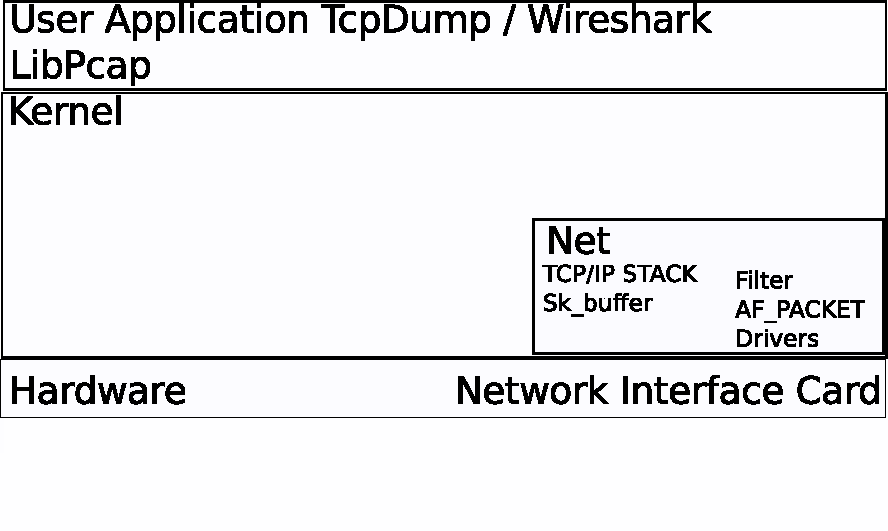
\includegraphics[scale=1]{pcap_architecture3}
       \caption{Arquitectura do LibPcap}
      \label{fig:pcap_architecture}
\end{figure}

A arquitectura de rede do núcleo de sistema \textit{Linux}, utiliza \textit{socket buffers}, que contêm dados referentes às diferentes camadas da \textit{stack TCP/IP}.
Esta estrutura que dispõe de toda a informação sobre o pacote, a receber pela aplicação, é igualmente utilizada nos sistemas de monitorização em nível utilizador.
A monitorização da rede é efectuada directamente no controlador da interface de rede, utilizando para isso um \textit{socket} \textit{AF\_PACKET}.

A biblioteca dinâmica \textit{LibPcap} é utilizada pela generalidade dos programas de captura de pacotes.
Esta biblioteca, como é multi-plataforma, permite ao programador utilizá-la nos principais sistemas de operação, porque a \textit{API} da \textit{LibPcap} é opaca relativamente à implementação, esta sim, específica de cada plataforma.
Para ser possível efectuar a captura de pacotes, o programa tem de especificar qual a interface de rede que quer monitorizar.
Se necessitar de filtrar pacotes, especificará os filtros a utilizar, recorrendo para isso à função \textit{setFilter}, que aplicará o filtro criado anteriormente, através da notação \textit{BPF}.
Após esta inicialização, o programa poderá utilizar \textit{Polling}, de forma a obter os pacotes e analisá-los.


O módulo \textit{AF\_PACKET} permite utilizar explicitamente o modo promiscuo, ou seja permite que sejam capturados pacotes que não são destinados à máquina utilizada.
Na versão actual do núcleo de sistema do \textit{Linux} (2.6.32), o módulo \textit{AF\_PACKET} já pode utilizar um sistema de partilha de \textit{buffer}, com o espaço de utilizador.
Neste caso cabe ao utilizador definir explicitamente a forma como pretende utilizar o \textit{socket}. 
Para atingir este objectivo o utilizador tem de pedir ao núcleo, uma região de memória, sendo esta, posteriormente indicada como argumento de configuração do novo \textit{socket}.

Como o referido anteriormente, o \textit{AF\_PACKET}, permite a comunicação directa com o controlador da interface de rede, possibilitando capturar os diversos pacotes ainda antes destes poderem ser filtrados pela \textit{firewall}, presente no núcleo de sistema, neste caso o \textit{netfilter}.
Podem ser aplicados filtros aos \textit{sockets} de modo a aumentar a eficiência na captura dos pacotes, excluindo aqueles que são irrelevantes para a monitorização.

Dos filtros em questão merece especial referência:

\subsubsection{Linux Socket Filtering}
O \textit{Linux Socket Filtering} é derivado do \textit{BPF (Berkeley Packet Filtering)} que é o standard de \textit{de facto} para a criação de filtros dentro do núcleo de sistema. 

Este sistema de filtros permite aos os utilizadores com permissões de \textit{Super User}, definir filtros e afectá-los aos \textit{sockets}.
Os filtros definidos são descritos numa linguagem simples, de forma a efectuarem com rapidez a selecção dos pacotes a capturar, rejeitando todos os outros.
Se o filtro for demasiado complexo, não poderá ser aplicado no núcleo, sendo apenas possível aplicá-lo em nível utilizador, perdendo algum desempenho.
A linguagem utilizada para a criação dos filtros é traduzida para o \textit{Instruction Set}, definido no \textit{BPF}.
Este \textit{Instruction Set} utiliza operadores lógicos de forma a combinar as regras definidas nos filtros, criando-se apenas um filtro a ser aplicado aos pacotes.
Para se poder definir uma nova instrução no \textit{Instruction Set}, é necessário alterar o ficheiro \textit{grammar.y}, na entrada correspondente à posição que deverá ocupar na \textit{AST (Abstract Sintax Tree)}, e modificar as funções de criação do novo filtro, quer em modo utilizador quer dentro do núcleo de sistema.
Este desenvolvimento tem de ser efectuado par-a-par, pois a ser efectuado apenas de um lado, o outro tornar-se-á incompatível.~\cite{Mccanne92thebsd}.

\subsection{Limitações e optimizações}
De forma a medir o desempenho da \textit{LibPcap}, é frequente utilizar-se uma métrica que nos permita determinar a percentagem de pacotes que é possível capturar, sem que se verifiquem perdas.
Esta métrica é calculada sabendo o número de pacotes que atravessam um determinado \textit{router ou switch}, e compará-la com o número de pacotes capturados na interface.
Uma variante desta medida de desempenho é combiná-la com o máximo número de regras que é possível aplicar, sem que se assista à perda de pacotes.
É particularmente importante conhecer o número máximo de pacotes capturados ou regras aplicáveis aos filtros, afim de determinar a velocidade máxima expectável de captura.
Quanto mais eficiente for a filtragem, menor o número de pacotes transferidos para as aplicações, o que se traduz numa menor sobrecarga para o sistema, aumentando o seu desempenho.

\paragraph{Captura de pacotes com \textit{TimeStamp}}
% como etiquetar os pacotes 
Um dos pontos que pode influenciar negativamente o desempenho da obtenção de pacotes, sem que contudo seja significativo, é a necessidade de colocar nestes, uma estampilha temporal, com o tempo da sua chegada ao sistema.
O \textit{LibPcap} pode obter estes dados de duas formas distintas, dependo da interface de rede que esteja a ser utilizada.
Se a interface de rede fornecer a estampilha temporal associada ao pacote, o \textit{LibPcap} pode utilizar este valor, caso contrário será necessário obter a estampilha temporal da chegada do pacote ao sistema.
A forma de obtenção da estampilha pela \textit{LibPcap}, processa-se através da função \textit{gettimeofday}.

\subsubsection{Implementações que permitem um aumento da taxa de transferência}

Apesar da \textit{API} da \textit{LibPcap} ser igual em diferentes plataformas (\textit{Windows}, \textit{Linux}, \textit{FreeBSD}, etc), o desempenho desta pode variar.
Quando exista pouco tráfego de rede estas diferenças são pouco notórias, mas logo que este se intensifica, estas acentuam-se bastante, como demonstra o estudo \textit{Improving Passive Packet Capture: Beyond Device Polling} \cite{Deri2004}.

Diversos esforços no sentido de aumentar o desempenho da captura de pacotes têm sido efectuados.
Relativamente ao \textit{software}, são conhecidos esforços na utilização da técnica de \textit{mmap}, de forma a reduzir o número de cópias de dados entre as aplicações e o núcleo de sistema.
Igualmente no \textit{hardware}, tem-se assistido a uma evolução no sentido de reduzir as interrupções efectuadas ao cpu, adicionando nas interfaces de rede processadores dedicados às funcionalidades presentes no núcleo, de modo a libertá-lo da execução destas tarefas.

\paragraph*{NAPI}

A utilização desta nova \textit{API} permite diminuir o número de trocas de contexto entre o controlador da interface e o núcleo de sistema.
Sempre que o cpu atende uma interrupção de rede, obtem um número maior de dados, que combinado com um sistema de memória partilhada aumenta substancialmente o desempenho.
Esta técnica encontra-se descrita na sub-secção \ref{par:NAPI}

\paragraph*{PACKET\_MMAP}

Com base na técnica \textit{MMAP} descrita em \ref{par:MMAP_overview}, foi criado o \textit{PACKET\_MMAP}, disponível a partir da versão 1.0.0 da biblioteca do \textit{LibPcap}.
Este módulo permite algumas melhorias em termos de desempenho, visto que foi reduzido o número de cópias efectuadas e de trocas de contexto, face à anterior versão 0.9.8 da biblioteca \textit{LibPcap}.

Para além destas modificações no \textit{Packet\_MMAP}, o núcleo de sistema de operação \textit{Linux} na sua versão 2.6, passou a contar com a nova \textit{API} de rede (\textit{NAPI}).

Se as interfaces de rede suportarem um mecanismo de mitigação de interrupções, é possível obter melhores resultados, conforme \cite{Deri2004}.

\paragraph*{PF\_RING}

Este é um novo módulo para o núcleo de sistema, criado com base em duas técnicas \textit{mmap} e \textit{ring\_buffers} anteriormente descritas.

Este módulo difere na abordagem utilizada no \textit{Packet\_MMAP}, porquanto nesta a memória é mapeada entre a ferramenta e o controlador da interface, enquanto que no \textit{Packet\_MMAP} a memória é mapeada entre a ferramenta e um \textit{buffer} externo ao controlador da interface, mas interno ao núcleo de sistema.
Esta abordagem permite que os dados fiquem disponíveis para a aplicação directamente, verificando-se a inexistência de cópia dos dados do \textit{buffer} do controlador, para o \textit{buffer} partilhado entre a ferramenta e o núcleo\cite{:PF_RING}.
 
\paragraph*{PF\_RING com DNA (Direct NIC Access)}
Baseando-se na técnica anteriormente descrita de utilizar um \textit{buffer} partilhado entre a ferramenta de monitorização e o controlador, assiste-se a uma evolução desta técnica, ao permitir que a interface de rede partilhe um \textit{buffer} com a ferramenta de monitorização, possibilitando que os pacotes passem directamente para esta.\cite{:IntroPF_RIDNADirecNICAcces}.
Esta partilha é efectuada utilizando \textit{mmap}, \textit{ring\_buffers} e \textit{DMA}.
Para se utilizar esta técnica é necessário que a interface de rede, permita a utilização de memória partilhada e \textit{DMA}.

\paragraph*{Sistemas \textit{multi-core} e multi-processador}

Com o aparecimento de sistemas \textit{multi-core} e \textit{multi-processador} a que a generalidade do público tem acesso, a paralelização de código ou a forma de tirar partido destas arquitecturas, que permitem um melhor aproveitamento dos recursos, assumem uma particular importância.
De forma a tirar partido das arquitecturas \textit{multi-core}, é necessário que o controlador e interfaces de rede, os \textit{buffers}, e os controladores de \textit{DMA} (\textit{Direct Memory Access}), sejam modificados de forma a conhecerem esta estrutura.
É pois, determinante um esforço conjunto envolvendo todas estas componentes, com vista à obtenção do máximo rendimento destas arquitecturas\cite{Deri:2010}.

\subsection{Formas de melhorar a filtragem}
 O dinamismo das aplicações, nomeadamente das aplicações multimédia, deu origem a diversos estudos sobre a forma de monitorização de rede, que estas necessitam.
Estas aplicações utilizam diversos fluxos de dados, designadamente de transmissão e de recepção.
Em geral, as aplicações multimédia, com base na \textit{internet} utilizam uma metodologia cliente/servidor, onde o servidor aguarda pedidos do cliente num determinado porto.
O cliente, conhecendo antecipadamente este porto, liga-se.
A partir deste ponto, iniciam-se trocas de informações que irão originar a troca de portos dinâmicos e posteriormente o processo de transmissão/recepção de dados multimédia.

As aplicações multimédia assentes na \textit{internet} são apenas um exemplo de aplicações com diversos fluxos, em que as portas de comunicação entre as aplicações, são negociadas dinamicamente.

Como o referido em \ref{sect:LibPcap}, a captura de pacotes é definida em filtros estáticos e para capturar este tipo de tráfego, é necessário modificar os filtros definidos, de modo a acompanhar o protocolo.
Esta forma de captura mostra-se bastante ineficaz, o que motivou a que fossem estudadas algumas alternativas, tendo em vista a correcção desta situação.
Os projectos \textit{mmdump}\cite{505678}, %\textit{Fairly Fast Packet Filters (FFPF)}\cite{1251278} 
e \textit{Swift}\cite{1387609} são dois destes casos estudados, que merecem especial relevância e que adiante se analisam:

\paragraph*{MMDump - } É uma ferramenta de monitorização de protocolos multimédia com suporte na rede.
Esta aplicação tem como base o \textit{tcpdump}, sendo a captura de pacotes efectuada através da utilização de filtros.
Para determinar os portos a obter, é necessário analisar o conteúdo dos pacotes direccionados a portos específicos, e a partir destes é possível identificar os novos portos negociados dinamicamente pela aplicação, e proceder à alteração dos filtros a aplicar.
Como a alteração, que é constituída pela cópia do novo filtro para o núcleo e verificação de segurança, de forma a validá-lo, é um processo demorado, é necessário reduzir este tempo, com o objectivo de ter uma aplicação que consiga minimizar o grau de perturbação no sistema.

Na alteração do filtro, foi verificado que existe um certo padrão, que consiste em pré-estabelecer uma parte comum a ser adicionada ao filtro, e apenas alterar a parte referente aos portos.

Esta forma de monitorização é muito específica, pelo que é imprescindível todo o protocolo interno de comunicação.
Assim, para cada novo protocolo a monitorizar, é necessário acrescentar um novo módulo com a interpretação desse protocolo.

% \paragraph*{\textit{Fairly Fast Packet Filter} (FFPF)}

\paragraph*{\textit{Swift} - }
É uma ferramenta de criação de filtros, cujo principal objectivo é a melhoria do desempenho da utilização destes, na captura do tráfego de rede.
Nesta ferramenta, foi avaliado o tempo de alteração dos filtros, utilizando o \textit{Linux Socket Filtering}, pois estes são os filtros de referência no sistema de operação \textit{Linux}.
A aplicação destes filtros a partir da biblioteca \textit{LibPcap} compreende três fases: cópia do filtro definido em nível utilizador para o núcleo de sistema, verificação de segurança, e aplicação do filtro.
De forma a diminuir a latência de actualização dos filtros, foi criada uma especificação de modo a que estes não necessitassem de ser analisados relativamente à segurança, visto que a própria linguagem garante as propriedades de segurança necessárias.
Com este novo \textit{instruction set}, e sem necessidade de verificação, foi reduzida a latência de actualização dos filtros, o que conduziu a um aumento de desempenho na utilização de filtros dinâmicos.

\section{Captura de tráfego de um processo utilizando monitorização da estrutura de rede}
\label{sect:outras_abordagens}

A captura do tráfego respeitante a um processo, foi alvo de estudo em \cite{1688981} e em \cite{Farruca:2009}, esta última objecto de uma dissertação de mestrado.

No primeiro trabalho, foi desenvolvido um sistema de captura de pacotes de um determinado processo, utilizando um módulo no núcleo de sistema que intercepta e captura os pacotes do processo.

Este sistema é constituido por três componentes essenciais, uma dentro do núcleo de sistema e duas em nível utilizador.
Na realização do trabalho, foi utilizada a ferramenta \textit{KProbes} para a monitorização de algumas funções do núcleo de sistema \textit{Linux}, de forma a conhecer quais os portos que vão ser utilizados por uma determinada aplicação.
Logo que obtida, a informação é enviada para um processo em nível utilizador que tem o registo de todos os portos que estão a ser utilizados pela aplicação objecto de monitorização.
Se esse porto não estiver a ser monitorizado, essa informação é passada a outro processo que utiliza a biblioteca \textit{LibPcap} de forma a capturar o tráfego existente nesse porto.


\begin{figure}[h!]
       \centering
       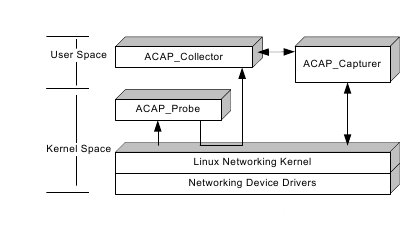
\includegraphics[height=2in]{captura_kprobes_paper}
       \caption{Arquitectura da monitorização de tráfego}
	\label{fig:paper_capture_kprobes}
\end{figure}


Analisando a arquitectura de monitorização de tráfego representada na figura~\ref{fig:paper_capture_kprobes}, o ACAP\_Collector e o ACAP\_Capturer, estão em nível utilizador, de onde se infere que o desempenho desta ferramenta é passível de ser aumentado, caso esta seja completamente implementada dentro do núcleo de sistema de operação.

Relativamente ao segundo trabalho, foram implementadas duas abordagens: uma com monitorização da aplicação e outra através de informações pertencentes ao núcleo do sistema de operação.
No que à primeira diz respeito, a monitorização efectuada processou-se através da interceptação das chamadas à bibiloteca \textit{LibC}, para a utilização de \textit{sockets}, criando uma bibiloteca partilhada com a mesma sintaxe das chamadas que são utilizadas.
A opção pela utilização deste método, implica definir a variável de ambiente \textit{LD\_PRELOAD}, de forma a operar esta intercepção.
Como esta biblioteca está em nível utilizador, mostra-se necessário capturar todos os pacotes e apenas em nível utilizador visualizar o tráfego respeitante ao processo.
Esta obrigatoriedade de capturar todos os pacotes pode constituir uma tarefa com elevado grau de perturbação do sistema.

No que à segunda abordagem se refere, o método de monitorização utilizado baseou-se na consulta efectuada de forma regular com intervalos reduzidos, dos dados referentes aos portos de comunicação, utilizados pela aplicação, que são exportados pelo núcleo através do \textit{ProcFs}.
Esta forma de monitorização consome demasiados recursos e não se mostra totalmente fiável, na medida em que quanto menor o intervalo de tempo utilizado, maior é a perturbação apresentada pelo sistema.

\section{Filtragem de pacotes de um processo através do \textit{Netfilter}}

O \textit{NetFilter} é o sistema de filtragem de pacotes do núcleo do \textit{Linux} que irá ser apresentado na secção \ref{}.
Foi implementado um módulo no núcleo utilizando o \textit{NetFilter} que filtra os pacotes pertencentes a um processo ou utilizador.
Este sistema, verifica relativamente a cada pacote que é recebido ou enviado, se este faz parte do processo ou processos pertencentes a um utilizador, verificando canal a canal se o identificador do canal do pacote é igual ao canal do processo.


Falta falar do ipt\_owner do iptables entre outros ....

